% !TeX root = ../main.tex

\chapter{以可佳机器人为基础的行人追踪与系统}

\section{视觉行人追踪系统}

\subsection{总体架构}

\subsubsection{目标人物注册}

  追踪系统在初始化时需要得到目标行人所在的大致位置,即提供行人在初始帧中的界限框(bounding box),并由此对追踪器和分类器进行初始化。为了能够有效地对目标用户进行识别,这里采用开源系统OpenPose\cite{cao2018openpose}来进行人体的骨骼识别。OpenPose系统不仅可以判断出图像中所有人物的骨骼信息,还可以对人物的姿势进行识别,这带来了另一个好处,即我们可以要求被跟随的目标站在机器人前方做出一个指定的姿势,如举起右手,直到机器人提示注册成功,这样一来,我们就可以在对目标人物的特征没有先验知识的情况下在初始化时发现目标了。

\subsubsection{行人追踪器}
  根据VOT2017的结果\cite{kristan2017visual},CSR-DCF算法在实时实验中取得了最佳的结果,由于其出色的性能和实时性的良好实现,选用CSR-DCF作为追踪器。CSR-DCF追踪器是一种相关滤波追踪器,它将HOG和颜色特征相结合,并提出了空间和通道置信度来对追踪器进行调整。在实际测试中,CSR-DCF算法可以达到约40FPS的帧率,达到实时性要求。相对于其他速度更快的算法,如MedianFlow、MOSSE、CamShift算法,CSR-DCF算法更为准确,在一定程度上对于遮挡鲁棒。帧率相对较高的KCF追踪器在尺度不变的情况下也能做到相似的准确程度,能在一定程度上解决目标被遮挡的问题,且有可能在失败后再次恢复,但前面已经讨论过,KCF算法无法适应目标尺度大小的变化。另一个适应于长期追踪的TLD算法,识别准确率较低,边界框会经常跳动或漂移,甚至会经常检测到错误的位置,但在目标在视野中消失一段时间后再回到画面时,TLD算法能识别到目标的回归并继续对其追踪。

  在实际使用时,CSR-DCF算法最大的缺点即为它几乎无法从跟踪失败中恢复,且对于错误的情况,CSR-DCF算法常常不能及时发现。既然选用了CSR-DCF算法,并想使用它来完成一个长期追踪的任务,这就成为了必须克服的问题。为此,在系统中加入一个分类器,该分类器在追踪时检测追踪器是否发生错误,并在追踪器追踪失败时尝试找回目标、帮助重新建立追踪。

\subsubsection{分类器}
\paragraph{分类器的选择}
  分类器通常要结合人工特征来使用,在行人识别中,最为常用的特征即为HOG特征。HOG特征和SVM分类器的组合从\citet{dalal2005histograms}最先提出开始,就在行人检测领域取得了重大的成果和最好的效果。但由于HOG检测的是人体的轮廓特征,对于形变和快速运动效果不好,当图像分辨率较低时效果也会变差。此外,HOG对于不同行人之间进行分辨效果也不佳。由于HOG特征的这些缺点,同时引入颜色直方图来对图像信息做补充。颜色直方图对光照变化和背景颜色相似的情况较为敏感,对目标的细节信息和颜色的相对位置不关注,但这些问题可以由HOG来代为弥补,而颜色直方图没有边界效应,对快速运动不敏感,且由于不同行人的衣着不同,对于不同行人的分辨也起到很大作用。所以在本文中使用HOG特征和HSV直方图中的H、S直方图结合起来描述目标的特征。

  为了分类精度,使用高斯核的SVM分类器进行分类。为了减少运行时计算量,且避免错误的追踪结果污染分类器的情况,这里仅仅对分类器进行一次初始化而不是采用在线学习的机制。

\paragraph{分类器的初始化}

  在训练分类器时,需要正负样本,负样本从图像背景中提取,正样本即为目前目标所在图像区域。为了增加样本的数量,提高分类器准确度,采用以下两个方法:
  
  a. 在建立起追踪后,提取一定数量的帧后再进行训练。如设定提取前100帧的图像,这个过程约为5秒时间,在这段时间内,假设追踪器不会出现错误且目标不会被遮挡;但如果在这段时间内,由于物体离开视野或严重变形等原因导致追踪器发生失败,则立即将收集到的正负样本传给分类器进行学习。

  b. 参考类似MIL追踪器的思想,通过将初始帧进行一定的旋转、位移、尺度变化等操作增加正样本数量。如随机将物体所在界限框平移不超过$10\%$的距离,旋转不超过$5^{\circ}$的角度,进行$5\%$以内的缩小或放大,取新的界限框在图像中的区域,或对原图像进行镜面翻转、高斯模糊等操作,将这些得到的新图像块加入正样本,便可以大大提高正样本的数目。取负样本时,通过在界限框之外随机取背景图像即可达到需要的数目。

\paragraph{检测和恢复追踪器的错误}
  由于运行分类器的速度要明显慢于运行追踪器的速度,并不会对每一帧追踪器的结果进行验证,而是每10帧左右将当前追踪器得到的图像块输入到分类器中得到一个分数,即它属于正样本的概率。设置一个阈值$fail\_thred$,当得分小于该阈值时,认为当前图像块非目标区域。但是在追踪任务中,经常会出现目标发生形变和被遮挡的情况,追踪器可以对这些情况在一定程度上鲁棒,但分类器就会对其此时的结果直接否定。针对这种情况,设置一个能容忍分类器报错的最大次数,当分类器连续报错超过此阈值时,认为追踪器出错,误追踪了其他对象,否则认为是目标短暂地发生了形变或受到了遮挡,不对追踪器进行更新。

  当判断追踪器发生错误或追踪器自身发生失败时,使用分类器对当前帧进行不同尺度上的全局扫描,进行目标行人的搜索。在这个过程中,记录全局扫描中得到的得分最高的图像块,若其得分超过一个阈值$positive\_thred$,则认为该图像块包含目标,否则确认目标丢失。


\begin{figure}[htb]
  \centering
  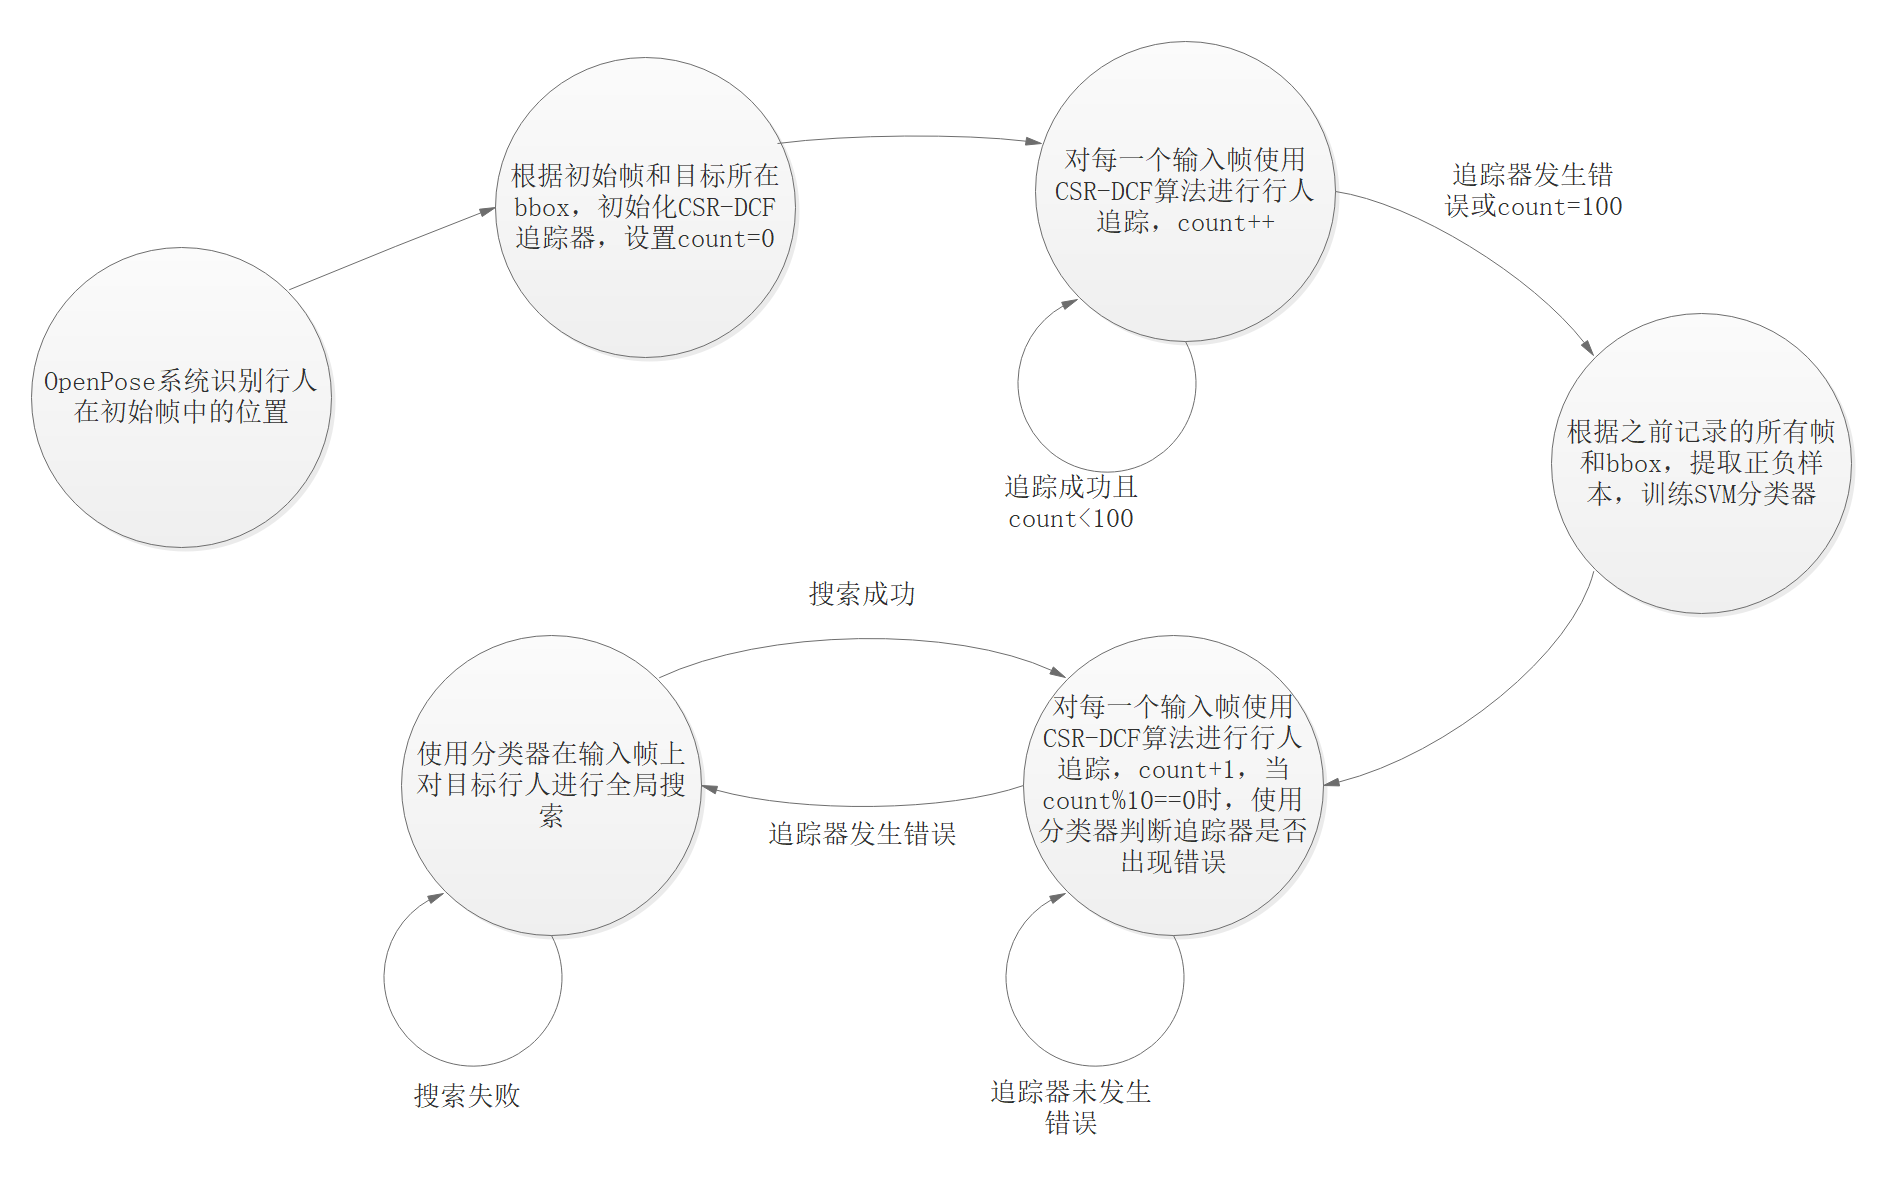
\includegraphics[width=1.1\textwidth]{statemachine.png}
  \caption{有限状态机}
  \label{fig:statemachine}
\end{figure}

\subsubsection{目标丢失恢复}

  当追踪失败且分类器也未能发现物体时,认为目标丢失,此时有几种可能:(1)目标从视野的左右两侧消失;(2)目标被完全部分或完全遮挡,如进入了另外的房间;(3)目标发生严重形变,或因光照的变化导致分类器检测失败。

  对于情况(1)和(2),相对于静态相机进行追踪时只能等待行人回到视野,机器人上的行人追踪系统可以使机器人主动转动视角或前往行人上一个出现的位置,来及时地恢复对行人的追踪。

  由于CSR-DCF追踪器几乎不能处理目标丢失后的恢复工作,使用分类器以一定频率对于输入帧进行全局扫描,当重新检测到目标时,重新初始化追踪器,建立追踪。


\subsubsection{总体结构}
  把初始化过程、追踪器、分类器三个模块整合起来,由一个有限状态机判断目标应采取的算法,如图\ref{fig:statemachine}所示。



\subsection{系统测试实验结果}

\begin{figure}[htb]
  \centering
  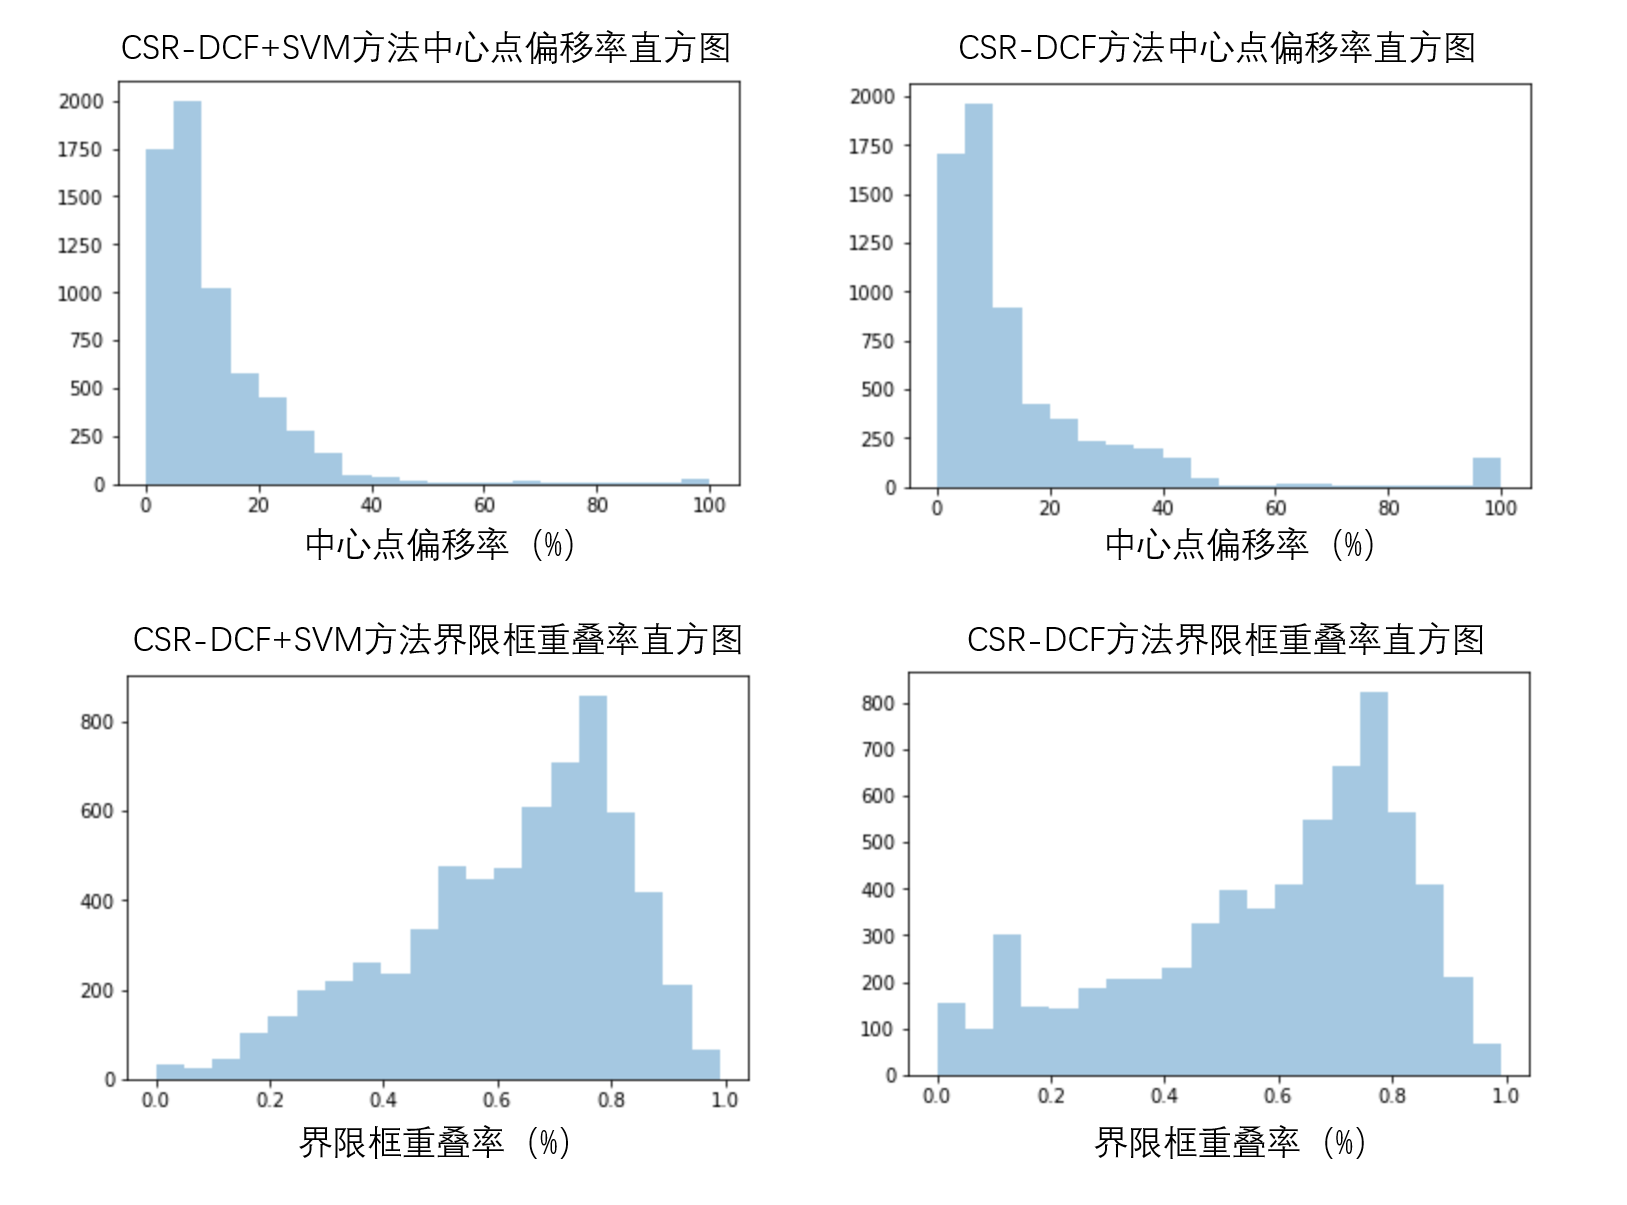
\includegraphics[width=1.0\textwidth]{result-histograms.png}
  \caption{CSR-DCF+SVM系统和CSR-DCF系统结果的中心点偏移率和界限框重叠率统计图}
  \label{fig:resulthistogram}
\end{figure}
\begin{figure}[htb]
  \centering
  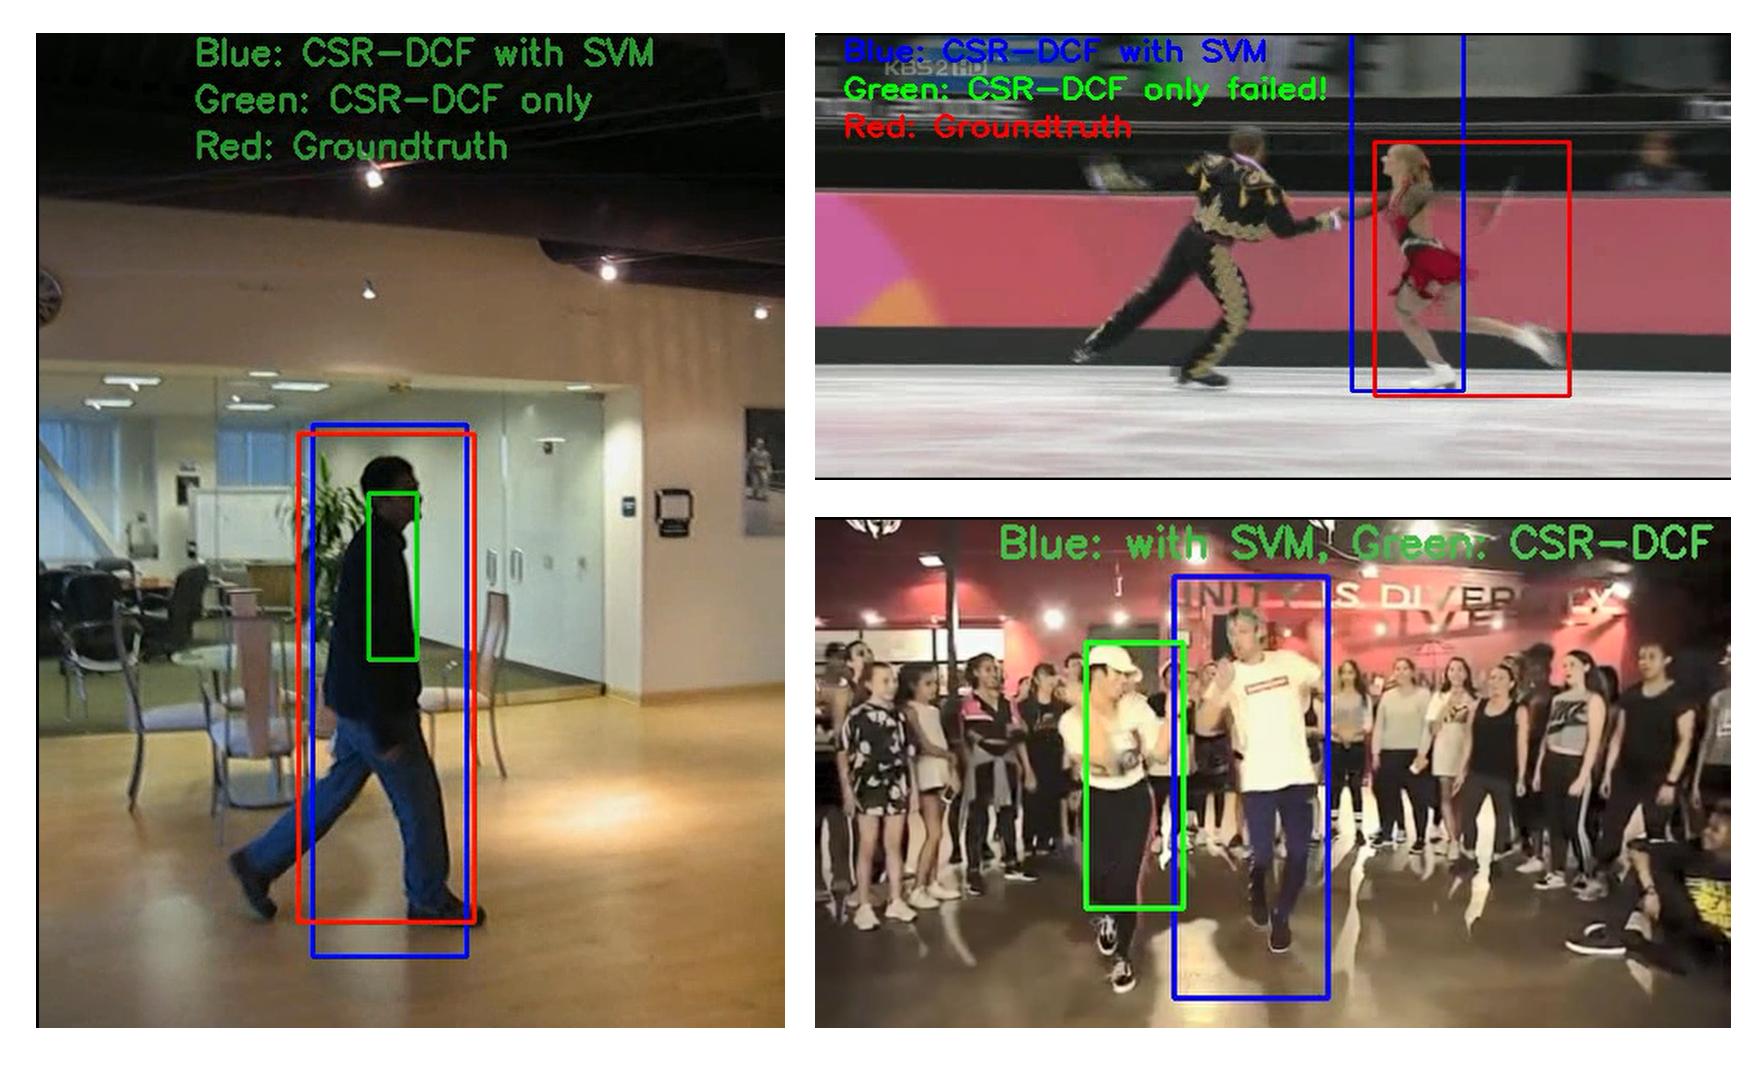
\includegraphics[width=0.9\textwidth]{samples.png}
  \caption{左:由于目标尺度变化导致CSR-DCF追踪器处于错误的尺度上;右上:由于目标运动速度过快导致CSR-DCF算法直接失败;右下:由于目标被另一个人物暂时遮挡导致CSR-DCF算法追踪了错误的行人。}
  \label{fig:samples}
\end{figure}

  使用目标检测和追踪数据集TB-100\cite{Wu2015Object}中的14个行人追踪视频序列进行测试,这14个视频囊括了包括光照变化、遮挡、目标变形、平面内旋转、平面外旋转、背景相似目标干扰、低分辨率、尺度变化、运动模糊、快速移动、低分辨率这些视频追踪中的常见难点。在测试中,分别统计追踪器得到的界限框与实际的重叠率,即两个界限框重叠区域的大小占它们总面积的比例,以及界限框中心点相对于实际界限框的偏移比例。由于在检测到目标区域后,接下来还会使用该区域的中心点作为目标的坐标控制机器人向其移动,所以使用中心点偏移衡量追踪和识别的精确程度,但由于中心点偏移率无法衡量追踪的尺度是否准确,所以另外引入重叠率。对于14个视频总共6448帧的图像,统计在每一帧上重叠率的平均值和重叠率超过50\%的帧数,以及中心点偏移率的平均值,偏移率超过50\%和20\%的帧数。为了验证加入分类器是否提高了系统准确度,还采用了只使用CSR-DCF追踪器的结果作为比较。

  在6448帧中,CSR-DCF+SVM系统出现了10帧的追踪失败,平均重叠率为62.16\%,有1625帧重叠率小于50\%;由于没有分类器帮助恢复,CSR-DCF系统的追踪失败则为141帧,平均重叠率为58.26\%,有2027帧的重叠率低于50\%。在中心点偏差方面,CSR-DCF+SVM系统的平均中心点偏差率为15.81\%,有108帧偏差率大于50\%,有82.74\%的帧中心点偏差率小于20\%;而CSR-DCF系统则有232帧的中心点偏差量超过50\%,77.73\%的帧中心点偏差率小于20\%,中心点偏差量平均值为27.32\%。具体的分布如图\ref{fig:resulthistogram}所示。


  实际上,在大部分情况下,由于CSR-DCF算法自身良好的性能,SVM对其的帮助有限,但在复杂情况下追踪失败,或者有遮挡情况下追踪器错误追踪了其他物体,由于尺度变化导致界限框处于错误的尺度等情况时,SVM便能对其提供有效地校正措施。如图\ref{fig:samples}所示。


  在追踪速度方面,在测试的14个视频上,单独使用CSR-DCF可以达到40.78FPS的平均帧率,而加入SVM后,平均帧率降为16.36FPS,勉强能够进行实时的使用。CSR-DCF+SVM系统的帧率收到视频质量的影响较大。当人物未收到遮挡或发生形变较小时,仅使用SVM来进行验证几乎不会影响视频帧率;而当SVM验证错误,或者追踪失败,而导致需要进行全局的扫描检测时,便会大大拖慢整体帧率。

\section{行人定位与机器人导航}

  通过视觉追踪系统获得行人在RGB图像中的位置,并不是对行人定位模块的终点。可佳机器人配备了Kinect深度相机,它可以同时为机器人提供RGB图像和深度图像的输入,经过对齐后,便可以简单地通过目标在RGB图像上的位置得到目标相对于机器人的角度和距离,从而得出目标的3D坐标。

  但Kinect的深度图像也有一定的不足。使用RGB-D相机Kinect作为彩色图像和深度信息的输入,而Kinect的深度图像只能有效判断80厘米之外的物体的距离,且由于Kinect通过红外发射器和红外摄像头来获得深度信息,所以受阳光照射的影响较大,所以在实际使用中,Kinect深度图像可能会出现不稳定和空洞现象。对于Kinect的深度图像在近距离精度较低的现象,可以考虑在较近距离内使用2D激光进行行人的3D位置判别。对于Kinect的空洞现象,由于视觉追踪系统最终得到的一个区域块,所以只需要从该区域块在深度图像中的对应区域中选择合适的深度信息即可,部分区域的噪音和空洞现象不会影响到最终的结果。

  在第三章中已经对ROS导航和可佳导航进行了调研,二者都有较为稳定鲁棒的导航功能。在得到目标的坐标后,可以选择调用ROS导航或可佳导航模块,将目的地实时地设置在行人目前所在位置,同时为了不妨碍行人的动作,还需要注意与行人保持一定的距离,在达到这个距离后停止机器人的移动。这样便可以实现一个较为稳定、交互友好的机器人行人跟随系统。